\subsection{Introducción:}

En este ejercicio realizaremos el \textit{scheduler}.

\begin{itemize}

\item [\textit{a)}]  Construir una función para inicializar las estructuras de datos del \textit{scheduler}.

\item [\textit{b)}] Crear la función  \textit{sched\_proxima\_a\_ejecutar()} que devuelve el  índice de la próxima tarea a ser ejecutada. 

\item [\textit{c)}]  Crear una función \textit{sched\_atender\_tick()} que llame a \textit{game\_atender\_tick()} pasando el número de tarea actual y luego devuelva el índice en la gdt al cual se deberá saltar. Reemplazar el llamado a \textit{game\_atender\_tick} por uno a \textit{sched\_atender\_tick} en el handler de la interrupción de reloj.

\item [\textit{d)}] Modificar la rutina de la interrupción 0x46, para que implemente los servicios según se indica en la sección 4.4.13

\item [\textit{e)}]  Modificar el código necesario para que se realice el intercambio de tareas por cada ciclo de reloj. El intercambio se realizará a según indique la función \textit{sched\_proxima\_a\_ejecutar().}

\item [\textit{f)}]  Modificar las rutinas de excepciones del procesador para que desalojen a la tarea que estaba corriendo y corran la próxima.

\item [\textit{g)}] Implementar el mecanismo de debugging explicado en la sección 4.8 que indicará en pantalla la razón del desalojo de una tarea.

\end{itemize}

\subsection{Ítem a): Inicializar el \textit{scheduler}}

Para incializar el scheduler completamos la funicón \textit{void sched\_inicializar()} del archivo sched.d. En el tp el scheduler es una estructura que posee un array de tareas denimoinado \textit{tasks} y un int denominado \textit{current} en el cual se guarda la tarea actual. Las tareas tambien son estructuras, y contienen un int para recordar la posicion en la que se guarda en la gdt y un puntero a la tarea que representan. Además le agregamos a esta estructura 3 ints, los cuales vamos a utilizar para saber lo siguiente: último jugador, último perro usado por el jugador A y último perro utilizado por el jugador B Esta estructura se puede obserbar en la siguiente imagen:

\begin{figure}[H]
\begin{center}
\minipage{0.5\textwidth}
 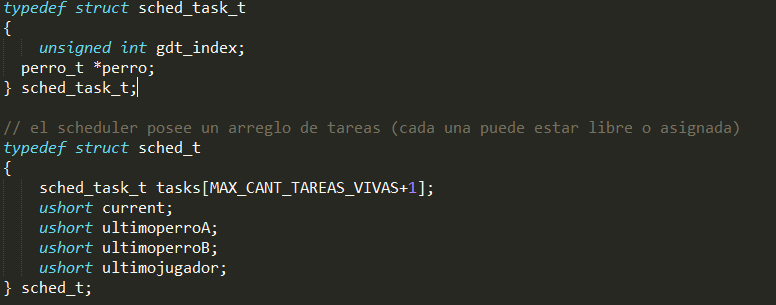
\includegraphics[width=\linewidth]{ejercicio7/sched.png}
 \caption{{\small Estructura del scheduler usado} }
\endminipage
\end{center}
\end{figure}

La función en cuestión es la siguiente:

\begin{figure}[H]
\begin{center}
\minipage{0.5\textwidth}
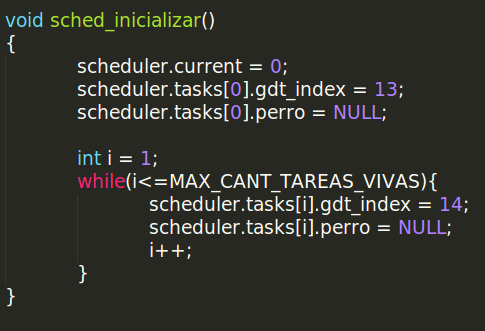
\includegraphics[width=\linewidth]{ejercicio7/funcion.png}
\caption{{\small \textit{void sched\_inicializar()} }}
\endminipage
\end{center}
\end{figure}

Para inicializar la estructura del scheduler realiza lo siguiente:

\begin{itemize}

\item [\textit{A}] Setea el valor de \textit{current} en 0, pues la tarea inicial debe ser la tarea \textit{IDLE} y por convención decidimos que esta se encuentre en la posición 0 del array de tareas. Devido a la decisión anterior, setiamos en el vector de tareas que el gdt\_index de la tarea 0 sea 13 (posición en la \textit{GDT} de la tarea \textit{IDLE} ) y que el puntero a la tarea de la tarea 0 sea \textit{NULL}.

\item [\textit{B}] Setea los 3 ints que agregamos en 0 ya que nadie jugo todavía.

\item [\textit{C}] Luego itera por todo el array de tareas \textit{tasks} seteandole a cada tarea una posición en la gdt correspondiente y seteando el puntero decada una en \textit{NULL}.

\end{itemize}

\subsection{Ítem b):  Crear la función  \textit{sched\_proxima\_a\_ejecutar()}}

Esta función comienza guardando cual es el jugador de la tarea actual y busca las siguiente tarea que corresponda al siguiente jugador. Para eso se fija cual fue el último perro usado por el jugador contrario e itera por todos los perros de este a partir del último utilizado. Si no llega a encontrar ningun perro empieza a iterar por los perros del jugador actual, tambien empezando a iterar desde el último perro utilizado por el jugador actual. Notar que para lograr esta forma de cambiar las tareas necesitabamos agregar los 3 ints que aclaramos al principio.


\subsection{Ítem c):  Crear una función \textit{sched\_atender\_tick()}}

Esta función debería devolver la posicion de la \textit{GDT} de la proxima tarea, para eso utiliza la funcion del ítem anterior, además actualiza el int \textit{current} de la estructura del sheduler y actualiza cual fue el último jugador y su último perro utilizado.

\begin{figure}[H]
\begin{center}
\minipage{0.8\textwidth}
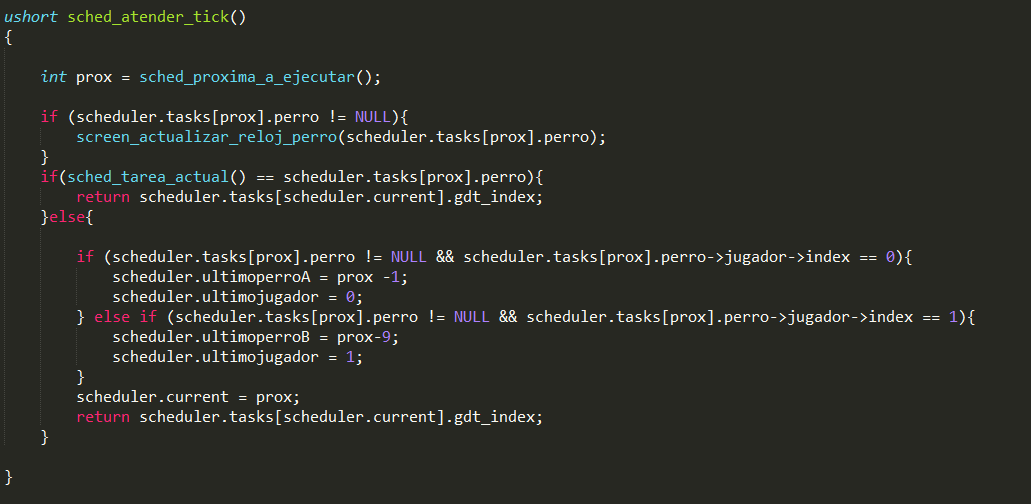
\includegraphics[width=\linewidth]{ejercicio7/atendtick.png}
\caption{{\small \textit{Funcion proxima tarea a ejecutar }}}
\endminipage
\end{center}
\end{figure}

\subsection{Ítem d):  Atender la interrupcion 0x46}

Explicado en el ejercicio 6, ítem h, es igual solo que ahora no se ignora el jmp a la tarea $idle$

\subsection{Ítem e):  Realiza el intercabio e tareas}

El intercambio de tareas lo realizamos en cada interrupción del reloj, utilizando las funciones explicadas anteriormente. Para utilizarlas escribimos las siguientes lineas en la \textit{RAE} del reloj:

\begin{center}

    pushad \\    
    call fin\_intr\_pic1 \\
    call sched\_tarea\_actual \\
    push eax    \\
    call game\_atender\_tick \\           
    call sched\_atender\_tick \\

    shl ax, 3  \\
    str cx \\
    cmp ax,cx \\
    je .fin \\

    mov [sched\_tarea\_selector], ax \\
    jmp far:[sched\_tarea\_offset] \\

    .fin: \\
     call screen\_actualizar\_reloj\_global \\    
    pop eax \\
    popad \\
    iret \\

\end{center}

Esta rutina pregunta por la poscicion de la \textit{GDT}  de la proxima tarea a ejecutar y si la proxima tarea a ejecutar es la misma que se esta ejecutando ahora no hace nada, sin embargo si es diferente realiza un \textit{jmp far} utilizando como selector la posicion en la \textit{GDT} correspondiente. De esta forma se  guarda la \textit{TSS} actual y se carga la nueva. \\

A esta rutina luego le agregamos más código para ver si el juego estaba frenado porque el modo debug había detectado que un perro habia generado una falta. No lo mostramos en este punto para que quede mas claro, además el modo debug no influye en este ítem.

\subsection{Ítem f):  Realiza el mecanismo de debug}

Para este ítem realizamos varias cosas:

\begin{itemize}

\item[A]: Creamos dos variables, $juegoFrenado$ y $modo_debug$, la primera vale 0 por defecto y pasa a valer 1 cuando el modo debug esta activado y se detecta que un perro causo una falta, sirve para que si esta prendida, la rutina del reloj salte siempre a la tarea $idle$. La segunda simplemente indica si el modo debug esta activado o no, si esta activada el juego se pone en pausa y muestra la pantalla debug cuando un perro rompe el programa, sino, esta pantalla no se muestra y simplemente se elimina el perro.

\item[B]: Modificamos la $RAE$ correspondiente a las primeras 20 interrupciones, para que de esta forma, en vez de hacer simplemente jmp \$ salte a la funcion $set_frenado()$.

\begin{figure}[H]
\begin{center}
\minipage{0.8\textwidth}
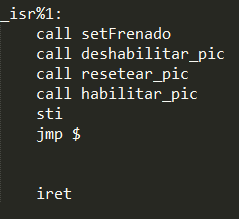
\includegraphics[width=\linewidth]{ejercicio7/isr.png}
\endminipage
\end{center}
\end{figure}


\item[C]: Creamos la funcion $set_frenado()$ la cual se fija si el modo debug esta activado, si lo esta, pone la variable $juegoFrenado$ en 1 e imprime la pantalla debug. Si el modo debug no esta activado simplemente elimina la tarea actual, la cual es la que rompió el juego. De esta manera el juego puede continuar.

\begin{figure}[H]
\begin{center}
\minipage{0.8\textwidth}
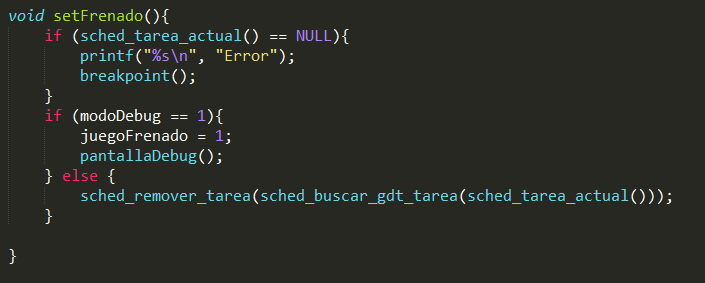
\includegraphics[width=\linewidth]{ejercicio7/setfrenado.png}
\caption{{\small \textit{Funcion proxima tarea a ejecutar }}}
\endminipage
\end{center}
\end{figure}


\item[D]: Modificamos la rutina del reloj para que si la variable $juegoFrenado$ esta en 1, salte directamente a la tarea $idle$, sin hacer nada mas.

\begin{figure}[H]
\begin{center}
\minipage{0.8\textwidth}
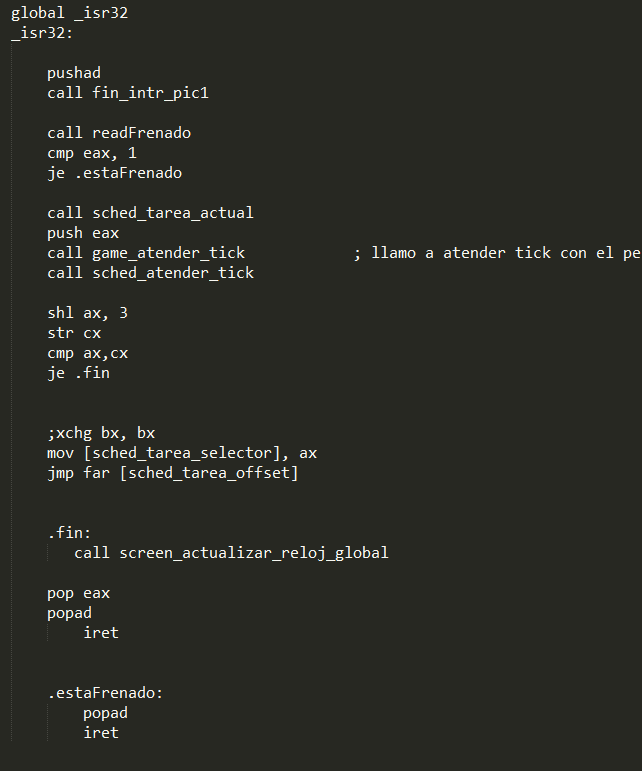
\includegraphics[width=\linewidth]{ejercicio7/reloj.png}
\endminipage
\end{center}
\end{figure}


\item[E]: Creamos la funcion $pantallaDebug()$ la cual guarda la pantalla y luego imprime por pantalla el contenido de todos los registros y parte del stack de la tarea.


\item[F]: Realizamos la funcion $continuarJuego()$ la cual se llama si se presiona la tecla $y$ y el juego estaba frendo. Esta función setea $juegoFrenado$ en 0, restaura la pantalla previamente guardada por $pantallaDebug$ y elmina la tarea actual. Ahora como el juego ya no esta frenado, se pueden saltar a otras tareas que no sean la $idle$.

\begin{figure}[H]
\begin{center}
\minipage{0.8\textwidth}
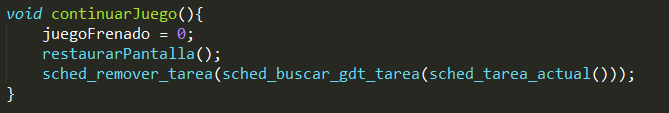
\includegraphics[width=\linewidth]{ejercicio7/continuar.png}
\endminipage
\end{center}
\end{figure}

\item[H]: Modificamos la $RAE$ del teclado, para que si el juego esta frenado solo se detecte la tecla y.

\begin{figure}[H]
\begin{center}
\minipage{0.8\textwidth}
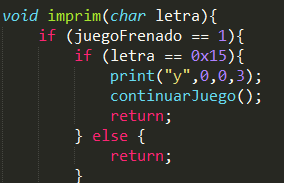
\includegraphics[width=\linewidth]{ejercicio7/teclay.png}
\endminipage
\end{center}
\end{figure}












